%%%%%%%%%%%%%%%%%%%%%%%%%%%%%%%%%%%%%%%%%%%%%%%%%%%%%%%%%%%%%%%%%%%%%%%%%%%%%
%%%                              Examples                                 %%%
%%%%%%%%%%%%%%%%%%%%%%%%%%%%%%%%%%%%%%%%%%%%%%%%%%%%%%%%%%%%%%%%%%%%%%%%%%%%%
\subsubsection{Examples}
\label{sec:opexamples}
The following example shows a possible \OPERATOR{} configuration:


\begin{boxedminipage}[t]{\linewidth}
\begin{alltt}
\OPERATOR
  \PROCESS
      AsmChar: \MATHEMATICA
    , Calculate: \BATCH \{"/usr/local/bin/doit -x -y"\}
    ;
  \FILESTREAM
      Input_Stream = file_in \{"Input Parameters", \FILTER="*.DAT"\}
    ;
  \REPORTSTREAM
      Calculation_Stream = report_out \{"Calculation Report"\}
    ;
  \PROCESSGROUP
       BatchProg \{"Batch Run"\}(
         bat_out = Calculate( bat_in );
       )
    ;
  \TASK
    BatchT \{"Optimize"\}\{
      Sn = 0;
      \WHILE( Sn < SnMax )\{
        \RUN BatchProg;
      \}
    \}
   ;
  \MENU
      Calculations
        ( \PROCESS BatchProg
        )
    ;
\END \OPERATOR;
\end{alltt}
\end{boxedminipage}


\newpage
\paragraph{\MESSAGEQUEUE{} \PUBLISH{} - \SUBSCRIBE{} example with \TIMER{}}
\label{sec:opexamples:messagequeue:publishsubscribe}

The following example shows a \PUBLISH{} - \SUBSCRIBE{} \MESSAGEQUEUE{} pattern. It also
shows the usage of \TIMER{}.

\vspace{1cm}
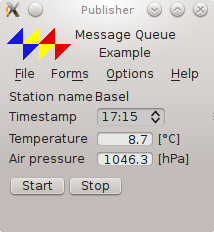
\includegraphics[valign=t]{examples/messageQueue/publisher}
\hspace{2cm}
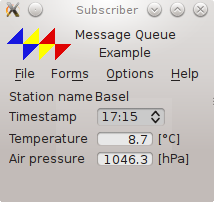
\includegraphics[valign=t]{examples/messageQueue/subscriber}
\vspace{1cm}

The example consists of four files:
\begin{itemize}
\item publisher.des  : INTENS application that publishes weather data using ZeroMQ.
\item subscriber.des : INTENS application that receives the published data.
\item common.inc     : Common code included in both publisher.des and subscriber.des.
\item timer.inc      : \TIMER{} code included in publisher.des.
\end{itemize}

\newpage
publisher.des:

\begin{boxedminipage}[t]{\linewidth}
\begin{alltt}
\DESCRIPTION "Publisher";

INCLUDE common.inc
INCLUDE timer.inc

\UIMANAGER
  \FORM
    main_form \{ \MAIN, \HIDECYCLE \} (
      weather_fg
    , timer_button_fg
    )
  ;
\END \UIMANAGER;

\OPERATOR
  \MESSAGEQUEUE
    weather_publisher \{
      \PUBLISH              // *MessageQueue Pattern
    , \PORT=5561            // TCP port
    \}
  ;
\END \OPERATOR;

\FUNCTIONS
  \FUNC
    publish_weather_func \{
      \PUBLISH (
        \MESSAGEQUEUE = weather_publisher
      , \HEADER="Weather"
      , \RESPONSE=weather_stream
      );
    \}
  ;

  \FUNC
    \INIT \{
      weather.stationName = "Basel";
      t = 0;
    \}
  ;
\END \FUNCTIONS;

\END.
\end{alltt}
\end{boxedminipage}


\newpage
subscriber.des:

\begin{boxedminipage}[t]{\linewidth}
\begin{alltt}
\DESCRIPTION "Subscriber";

INCLUDE common.inc

\UIMANAGER
  \FORM
    main_form \{ \MAIN, \HIDECYCLE \} (
      weather_fg
    )
  ;
\END \UIMANAGER;

\OPERATOR
  \MESSAGEQUEUE
    weather_subscriber \{
      \SUBSCRIBE            // *MessageQueue Pattern
    , \HOST="localhost"     // Hostname
    , \PORT=5561            // TCP port
    , (
        \HEADER="Weather"
      , \STREAM=weather_stream
      )
    \}
  ;
\END \OPERATOR;

\END.
\end{alltt}
\end{boxedminipage}


\newpage
common.inc:

\begin{boxedminipage}[t]{\linewidth}
\begin{alltt}
// Common parts of the message queue examples
\DATAPOOL
  \STRUCT
    Wheather \{
      \STRING
        stationName \{ \LABEL="Station name", \LABEL \}
      , timestamp   \{ \LABEL="Timestamp", \STRINGTIME \}
      ;
      \REAL
        temperature \{ \LABEL="Temperature", \UNIT="[°C]" \}
      , airPressure \{ \LABEL="Air pressure", \UNIT="[hPa]" \}
      ;
    \}
  ;
  Wheather weather;
\END \DATAPOOL;

\UIMANAGER
  \FIELDGROUP
    weather_fg (
      \LABEL(weather.stationName) weather.stationName \{ \COLSPAN=2 \}
    , \LABEL(weather.timestamp)   weather.timestamp   \{ \COLSPAN=2 \}
    , \LABEL(weather.temperature) weather.temperature:6:1
        \UNIT(weather.temperature)
    , \LABEL(weather.airPressure) weather.airPressure*1e-2:6:1
        \UNIT(weather.airPressure)
    )
  ;

  // Hide \STDWINDOW and \LOGWINDOW from \MAIN form
  \FORM
    stdwin_form \{ "Standard output", \HIDECYCLE
                , \CLOSEBUTTON=\NONE \} (
      \STDWINDOW \{ \SIZE=24*80 \}
    )
  , logwin_form \{ "Log output", \HIDECYCLE
                , \CLOSEBUTTON=\NONE \} (
      \LOGWINDOW \{ \SIZE=24*80 \}
    )
  ;
\END \UIMANAGER;

\STREAMER
  weather_stream \{ \JSON \} (
    weather
  );
\END \STREAMER;
\end{alltt}
\end{boxedminipage}


\newpage
timer.inc:

\begin{boxedminipage}[t]{\linewidth}
\begin{alltt}
// Timer parts for publisher.des
\DATAPOOL
  \REAL t;
  \STRING \{ \EDITABLE \}
    start \{ \LABEL="Start", \BUTTON, \FUNC=start_timer_func \}
  , stop  \{ \LABEL="Stop" , \BUTTON, \FUNC=stop_timer_func \}
  ;
\END \DATAPOOL;

\UIMANAGER
  \FIELDGROUP
    timer_button_fg (
      start   stop
    )
  ;
\END \UIMANAGER;

\OPERATOR
  \TIMER
    publish_weather_timer \{
      \FUNC=update_and_publish_weather_func
    \}
  ;
\END \OPERATOR;

\FUNCTIONS
  \FUNC
    update_and_publish_weather_func \{
      // update (simulate) weather data
      t += 0.1;
      weather.timestamp   = \CURRENTTIME;
      weather.temperature = 15 + \SIN(t) * 10;
      weather.airPressure = 102300 + \COS(t) * 3000;

      \RUN ( publish_weather_func );
    \}
  , start_timer_func \{
      \START (
        publish_weather_timer
      , \PERIOD=1
      , \DELAY=5
      );
    \}
  , stop_timer_func \{
      \STOP ( publish_weather_timer );
    \}
  ;
\END \FUNCTIONS;
\end{alltt}
\end{boxedminipage}
